\documentclass[tikz,border=10pt]{standalone}
% Shared look for every TikZ diagram. Load with % Shared look for every TikZ diagram. Load with % Shared look for every TikZ diagram. Load with \input{../../tools/tikz-style.tex}
\usepackage[T1]{fontenc}
\usepackage{lmodern}
\renewcommand{\sfdefault}{lmr}  % diagrams use the same serif as the text
\usetikzlibrary{arrows.meta, positioning, shapes.geometric, calc, fit, backgrounds}
\definecolor{cblue}{HTML}{4C78A8}
\definecolor{corange}{HTML}{F58518}
\definecolor{cgreen}{HTML}{54A24B}
\definecolor{cred}{HTML}{E45756}
\definecolor{cpurple}{HTML}{B279A2}
\definecolor{cgrey}{HTML}{6B6B6B}
\tikzset{
  every picture/.style={font=\sffamily, line width=1.2pt},
  box/.style={draw=#1, fill=#1!12, rounded corners=4pt, align=center, inner sep=7pt, minimum height=1.1cm},
  box/.default=cgrey,
  arrow/.style={-{Stealth[length=3mm]}, draw=cgrey, line width=1.4pt},
  title/.style={font=\sffamily\bfseries\Large},
  note/.style={font=\sffamily\small, text=cgrey, align=center},
}
\AtBeginDocument{\hyphenpenalty=10000 \exhyphenpenalty=10000}

\usepackage[T1]{fontenc}
\usepackage{lmodern}
\renewcommand{\sfdefault}{lmr}  % diagrams use the same serif as the text
\usetikzlibrary{arrows.meta, positioning, shapes.geometric, calc, fit, backgrounds}
\definecolor{cblue}{HTML}{4C78A8}
\definecolor{corange}{HTML}{F58518}
\definecolor{cgreen}{HTML}{54A24B}
\definecolor{cred}{HTML}{E45756}
\definecolor{cpurple}{HTML}{B279A2}
\definecolor{cgrey}{HTML}{6B6B6B}
\tikzset{
  every picture/.style={font=\sffamily, line width=1.2pt},
  box/.style={draw=#1, fill=#1!12, rounded corners=4pt, align=center, inner sep=7pt, minimum height=1.1cm},
  box/.default=cgrey,
  arrow/.style={-{Stealth[length=3mm]}, draw=cgrey, line width=1.4pt},
  title/.style={font=\sffamily\bfseries\Large},
  note/.style={font=\sffamily\small, text=cgrey, align=center},
}
\AtBeginDocument{\hyphenpenalty=10000 \exhyphenpenalty=10000}

\usepackage[T1]{fontenc}
\usepackage{lmodern}
\renewcommand{\sfdefault}{lmr}  % diagrams use the same serif as the text
\usetikzlibrary{arrows.meta, positioning, shapes.geometric, calc, fit, backgrounds}
\definecolor{cblue}{HTML}{4C78A8}
\definecolor{corange}{HTML}{F58518}
\definecolor{cgreen}{HTML}{54A24B}
\definecolor{cred}{HTML}{E45756}
\definecolor{cpurple}{HTML}{B279A2}
\definecolor{cgrey}{HTML}{6B6B6B}
\tikzset{
  every picture/.style={font=\sffamily, line width=1.2pt},
  box/.style={draw=#1, fill=#1!12, rounded corners=4pt, align=center, inner sep=7pt, minimum height=1.1cm},
  box/.default=cgrey,
  arrow/.style={-{Stealth[length=3mm]}, draw=cgrey, line width=1.4pt},
  title/.style={font=\sffamily\bfseries\Large},
  note/.style={font=\sffamily\small, text=cgrey, align=center},
}
\AtBeginDocument{\hyphenpenalty=10000 \exhyphenpenalty=10000}

\begin{document}
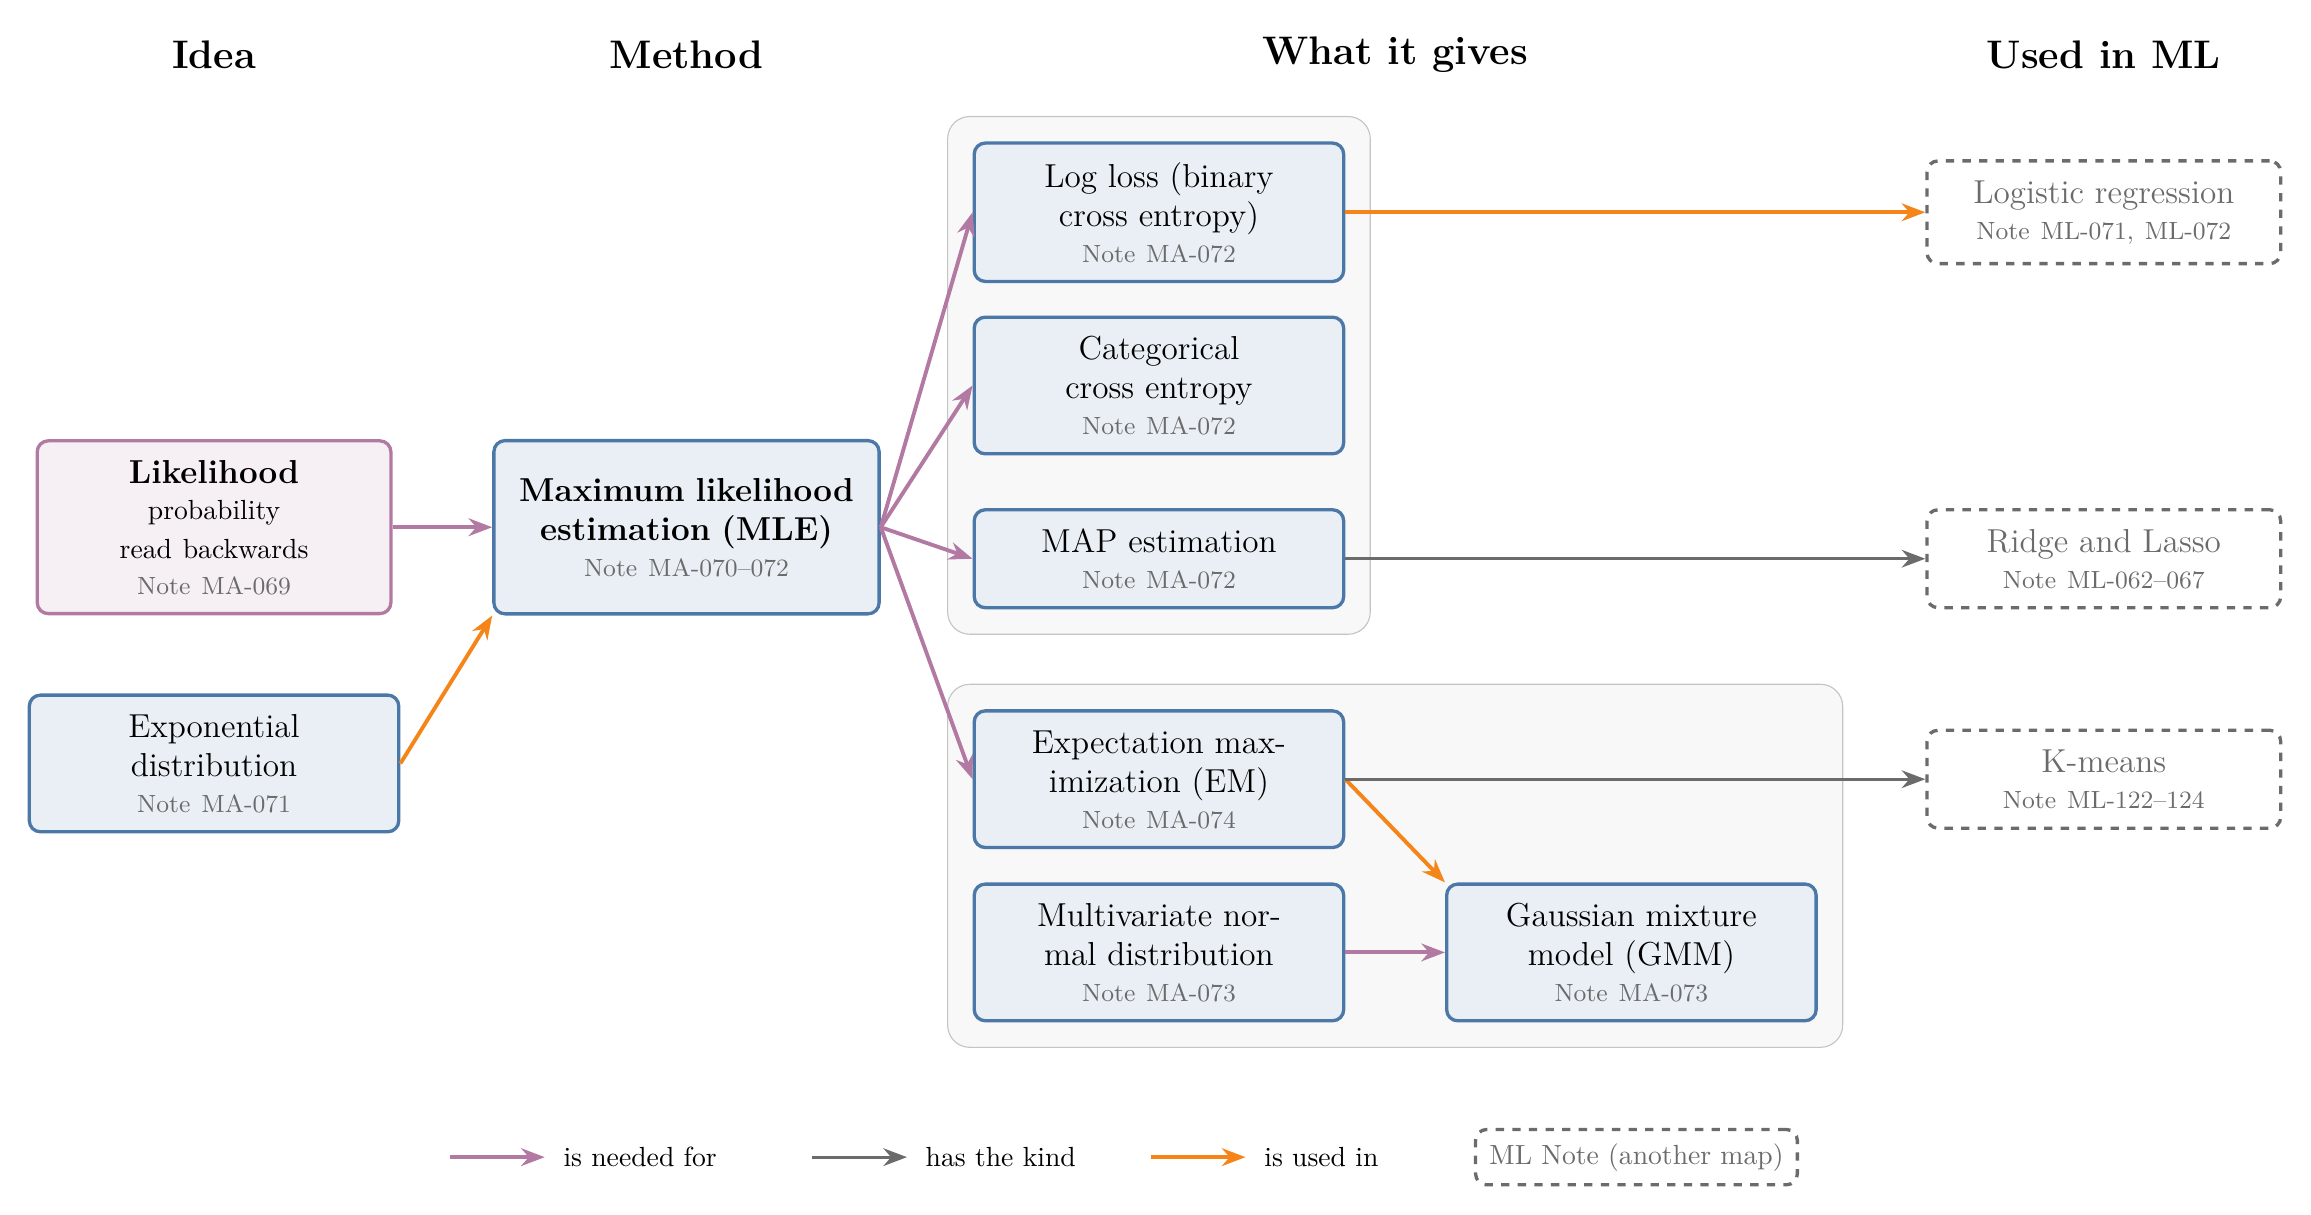
\begin{tikzpicture}[
    every node/.append style={font=\sffamily\large},
    idea/.style={box=cpurple, text width=4.0cm},
    con/.style={box=cblue, text width=4.2cm},
    prev/.style={draw=cgrey, dashed, rounded corners=4pt, align=center, inner sep=7pt, text=cgrey, text width=4.0cm, minimum height=1.1cm},
    group/.style={draw=cgrey!40, fill=cgrey!5, rounded corners=8pt, inner sep=9pt},
    needs/.style={arrow, draw=cpurple},
    kind/.style={arrow, draw=cgrey, line width=1pt},
    used/.style={arrow, draw=corange},
  ]
  \newcommand{\nt}[1]{\\[-1pt]{\small\color{cgrey}Note #1}}
  \node[title] at (0,11.6)  {Idea};
  \node[title] at (6,11.6)  {Method};
  \node[title] at (15,11.6) {What it gives};
  \node[title] at (24,11.6) {Used in ML};

  \node[idea] (lik) at (0,5.6) {\textbf{Likelihood}\\[-1pt]{\normalsize probability read backwards}\nt{MA-069}};
  \node[con] (exp)  at (0,2.6) {Exponential distribution\nt{MA-071}};
  \node[con, text width=4.4cm, minimum height=2.2cm] (mle) at (6,5.6) {\textbf{Maximum likelihood estimation (MLE)}\nt{MA-070--072}};

  % losses and priors
  \node[con] (ll)  at (12,9.6) {Log loss (binary cross entropy)\nt{MA-072}};
  \node[con] (ce)  at (12,7.4) {Categorical cross entropy\nt{MA-072}};
  \node[con] (map) at (12,5.2) {MAP estimation\nt{MA-072}};
  % mixtures
  \node[con] (em)  at (12,2.4) {Expectation maximization (EM)\nt{MA-074}};
  \node[con] (mvn) at (12,0.2) {Multivariate normal distribution\nt{MA-073}};
  \node[con] (gmm) at (18,0.2) {Gaussian mixture model (GMM)\nt{MA-073}};

  % ML uses
  \node[prev] (lr)  at (24,9.6) {Logistic regression\nt{ML-071, ML-072}};
  \node[prev] (rl)  at (24,5.2) {Ridge and Lasso\nt{ML-062--067}};
  \node[prev] (km)  at (24,2.4) {K-means\nt{ML-122--124}};

  \begin{scope}[on background layer]
    \node[group, fit=(ll) (ce) (map)] {};
    \node[group, fit=(em) (mvn) (gmm)] {};
  \end{scope}

  \draw[needs] (lik.east) -- (mle.west);
  \draw[used]  (exp.east) -- (mle.south west);
  \foreach \c in {ll, ce, map, em} \draw[needs] (mle.east) -- (\c.west);
  \draw[used]  (em.east) -- (gmm.north west);
  \draw[needs] (mvn.east) -- (gmm.west);
  \draw[used]  (ll.east) -- (lr.west);
  \draw[kind]  (map.east) -- (rl.west);
  \draw[kind]  (em.east) -- (km.west);

  % legend
  \begin{scope}[shift={(3.0,-2.4)}, every node/.style={font=\sffamily, anchor=west}]
    \draw[needs] (0,0) -- (1.2,0);     \node at (1.3,0) {is needed for};
    \draw[kind] (4.6,0) -- (5.8,0);    \node at (5.9,0) {has the kind};
    \draw[used] (8.9,0) -- (10.1,0);   \node at (10.2,0) {is used in};
    \node[draw=cgrey, dashed, rounded corners=4pt, inner sep=5pt, text=cgrey, anchor=west] at (13.0,0) {ML Note (another map)};
  \end{scope}
\end{tikzpicture}
\end{document}
